% !TeX root = ../main.tex

\chapter{相关研究综述}
\label{survey}

  \section{本章引言}
  \label{survey:introduction}
  基于IPv6源地址验证的用户身份识别与溯源技术是采用NIDTGA地址生成方案将用户身份信息通过加密手段嵌入至IPv6地址的后64位接口标识中,实现根据IPv6地址溯源使用该地址的用户身份的技术。其以网络层IPv6地址的真实性作为前提,由用户身份标识生成、用户认证、NIDTGA地址的生成与配置、根据NIDTGA地址追溯用户身份、网络管理员更新地址生成密钥等多个环节共同组成。用户身份识别与溯源系统的实现需要衔接上述各个环节,其安全性涉及到用户认证信息安全、IPv6地址安全、生成NIDTGA地址的密钥历史安全等方面。
  
  为了实现基于IPv6源地址验证的用户身份识别与溯源系统,将其部署落地并在全国高校进行推广应用,本文对网络层IPv6地址配置方式进行调研,以确认用户身份识别与溯源系统需要支持的地址配置场景。
  源地址验证技术作为用户身份识别与溯源系统的基础,其良好部署与安全性保障也直接影响到用户身份识别与溯源系统的正常运作,因此本章从接入子网、自治域内与自治域间三个层次分别对源地址验证的相关研究进行讨论。
  由于IPv6地址引入了有别于IPv4的新的地址配置方式,因此存在多种IPv6地址生成方案的研究,本文对各方案的侧重点进行讨论,其中包含用户身份识别与溯源技术所采用的NIDTGA地址生成方案。同时,对当前网络环境中常实施的用户身份认证手段进行介绍,并分析了常见溯源方案所存在的问题。此外,由于本文研究利用区块链提升用户身份识别与溯源系统及其基础技术的安全性,因此也对区块链技术的原理与发展现状进行了综述,为区块链方案的设计与实现提供指引。

  本章内容组织如下:第\ref{survey:configuration}节综述了IPv6地址的各种配置方式;第\ref{survey:sava}节根据SAVA体系结构的划分讨论各层次的源地址验证相关技术;第\ref{survey:generation}节描述了现有的IPv6地址生成方案,重点介绍了NIDTGA地址的生成方法;第\ref{survey:identity}节对现有的用户身份认证手段与溯源方案进行讨论;第\ref{survey:blockchain}节描述了区块链技术的发展现状;第\ref{survey:summary}节对本章进行总结。

  \section{IPv6地址配置方式的研究}
  \label{survey:configuration}
  IPv6地址的配置方式有三种,分别为:IPv6动态主机配置协议(Dynamic Host Configuration Protocol for IPv6,DHCPv6)\cite{RFC8415}、IPv6无状态地址自动配置(IPv6 Stateless Address Autoconfiguration,SLAAC)\cite{RFC2462}与IPv6静态配置。

  用户设备在接入网络时,根据接入子网网关设备周期性发送的路由器公告(Router Advertisement,RA)报文\cite{RFC2461,RFC5175}中的标志位来判断采用何种地址配置方式。RA报文中的Managed标志位与Other标志位被用于向用户设备告知子网的控制报文可达链路中存在可提供IPv6地址配置的DHCPv6服务器。RA报文中的Autonomous标志位则用于表示用户设备可采用SLAAC方式自动生成RA所公告IPv6前缀下的IPv6地址。

    \subsection{动态主机配置}
    \label{survey:configuration:DHCPv6}
    DHCPv6协议\cite{RFC8415}中定义了DHCPv6地址配置过程中涉及到的三种实体类型,DHCPv6客户端、DHCPv6中继与DHCPv6服务器。DHCPv6客户端一般由用户设备的操作系统内核提供;DHCPv6中继则由网络中的交换机或路由器等设备开启相应功能,负责将DHCPv6报文在不同链路之间进行中继转发;DHCPv6服务器负责集中管理其可提供的IPv6地址资源,响应用户设备的地址请求,根据自身策略选择可用的IPv6地址提供给用户,并设置租约时长等信息。由于DHCPv6服务器负责维护已配置的IPv6地址状态,因此若用户需要继续使用IPv6地址,则设备需要在DHCPv6服务器设置的租约时间到期前,向DHCPv6服务器发送续约报文以进行IPv6地址租约时间延长的请求。一个典型的DHCPv6地址配置流程如图\ref{fig:dhcpv6_no_relay}所示:
    \begin{enumerate}[1{)}]
      \item 首先,用户设备以组播地址FF02::1:2为目的地址,以自身的本地链路地址为源地址,发送Solicit报文,寻找可达链路中的DHCPv6服务器。
      \item DHCPv6服务器将在传输层547号端口监听用户设备或DHCPv6中继发送的DHCPv6报文,当收到Solicit报文时,其将根据自身的地址池状态与用户所在链路情况判断是否为请求的设备提供IPv6地址,若是,则向设备回复Advertise报文,其中包含DHCPv6服务器选择提供的IPv6地址、租约时间等信息。
      \item 用户设备收到若干个DHCPv6服务器回复的Advertise报文时,其将根据DHCPv6客户端的自身策略从其中选择一个IPv6地址,向其对应DHCPv6服务器发送Request报文,请求正式配置地址。
      \item 在收到Request报文后,若原先提供的IPv6地址仍有效,则DHCPv6服务器向用户设备回复一个Reply报文,其中包含此前Advertise报文所指定的各项信息;
      \item 用户设备收到最终的Reply报文后,根据其中包含的信息配置其网络适配器的IPv6地址,接入网络。
      \item 当IPv6地址租约中指定的T1时间到期时,用户设备将发送Renew报文,请求拓展IPv6地址租约时间。
      \item 在收到Renew报文后,若DHCPv6服务器检查状态后允许续约,则向设备回复Reply报文,指定新的租约时间,并更新自己维护的IPv6地址池状态。
    \end{enumerate}

    \begin{figure}[ht]
      \centering
      \subcaptionbox{无中继DHCPv6地址配置\label{fig:dhcpv6_no_relay}}
      {\includegraphics[height=5cm]{dhcpv6_no_relay.pdf}}
      \hspace{2em}
      \subcaptionbox{有中继DHCPv6地址配置\label{fig:dhcpv6_with_relay}}
      {\includegraphics[height=5cm]{dhcpv6_with_relay.pdf}}
      \caption{DHCPv6地址配置与续约流程}
      \label{fig:dhcpv6_configure}
    \end{figure}

    在实际的网络环境中,由于一个管理域中往往包含数量庞大的网络链路,为了管理的便利,通常只部署二到三台DHCPv6服务器,而不是在每一个链路中均进行部署,因此DHCPv6协议还支持如图\ref{fig:dhcpv6_with_relay}所示的中继机制:
    
    \begin{itemize}
      \item 对于Solicit、Request、Renew等由DHCPv6客户端发出的报文,DHCPv6中继将其作为Relay Forward报文中的中继报文选项Option 9所携带的值,并根据DHCPv6中继的配置设置其他一些选项,如设备的源MAC地址等,然后将Relay Forward报文组播发送到其他链路中;
      \item 对于Advertise、Reply等由DHCPv6服务器发出的报文,DHCPv6中继将其作为Relay Reply报文中的中继报文选项Option 9所携带的值,并根据配置设置其他的选项,然后将Relay Reply报文发送到对应链路中。
    \end{itemize}

    DHCPv6报文通过IETF标准定义的选项携带DHCPv6配置时的相关信息,较为重要的有DHCPv6唯一标识符DUID(DHCPv6客户端为Option 1,DHCPv6服务器为Option 2)、非临时IPv6地址与租约时间(Option 3)等信息。DHCPv6中继也可在封装后的中继报文中添加选项,比如Subscriber-ID选项(Option 38)\cite{RFC4580}携带在网络发生变化时保持不变的设备独立标识、Client Link-Layer Address选项(Option 79)\cite{RFC6939}携带用户设备的链路层地址等。

    由于DHCPv6协议采取集中式的地址管理方式,管理者可根据需要自主选择为用户设备分配的IPv6地址,并且其有状态的地址配置有利于管理者对用户设备上网行为进行管理,方便地址资源的管理和策略定制。

    \subsection{无状态地址自动配置}
    \label{survey:configuration:SLAAC}
    SLAAC协议\cite{RFC2462}与DHCPv6协议不同,没有一个集中式的服务器控制IPv6地址资源的分配,而是通过RA报文宣告IPv6地址前缀与SLAAC地址配置方式,告知用户设备使用相应的IPv6地址前缀生成IPv6地址进行配置。一个典型的SLAAC地址配置场景如图\ref{fig:slaac_configure}所示:
    \begin{enumerate}[1{)}]
      \item 网关设备向用户设备发送路由器公告RA报文,置位Autonomous标识位,包含可配置的IPv6前缀等信息。
      \item 用户设备根据自身选择的IPv6地址生成算法,一般采用EUI-64,生成IPv6地址的后64位接口标识,与RA报文中的IPv6前缀进行拼接,形成IPv6单播地址作为设备的试验地址。
      \item 用户设备在生成试验地址后将随机延迟一段时间,构建邻居请求(Neighbor Solicitation,NS)报文,以试验地址作为NS报文探测的目标地址,将其向试验地址所述的Solicited-Node组播地址发送以进行重复地址检测。
      \item 同一Solicited-Node组播组的其他节点收到NS报文后,检查其中目标地址是否与自身配置或正在试验配置的IPv6地址相冲突;若与自身已配置的地址相冲突,则向源设备回复宣告已持有该IPv6地址的邻居公告(Neighbor Advertisement,NA)报文;若与自身正在试验配置的IPv6试验地址冲突,则进行退让处理,不发送NA报文,重新生成IPv6地址进行试验配置。
      \item 若用户设备在等待时间内未收到其他节点发来的、以相同IPv6地址为目标地址的NS报文或NA报文,则重复地址检测成功,设备为其网络接口配置该IPv6地址,并设定网关地址等信息。
    \end{enumerate}

    \begin{figure}[ht]
      \centering
      \includegraphics[width=0.9\textwidth]{slaac_configure.pdf}
      \caption{SLAAC地址配置与重复地址检测流程}
      \label{fig:slaac_configure}
    \end{figure}

    SLAAC方式地址配置流程简单,不需要DHCPv6服务器的介入,但这种简单性导致了用户所使用的IPv6地址不受网络管理者的控制,因此难以对用户设备的地址选择策略进行定制和精细化控制,一些复杂的主机配置信息也难以通过这种方式进行传递。

    \subsection{静态配置}
    \label{survey:configuration:manual}
    IPv6静态配置方式通过人工向配置文件中写入IPv6地址、子网网关地址、DNS服务器地址等信息完成对用户设备的配置。静态配置的方式由配置人员在线下向网络管理员确定网络的配置信息,因此网络管理者也可以对其地址分配策略进行定制,实现较为精细的管理,但同时也需要对向用户设备提供接入功能的网络设备进行相应的配置以避免用户伪造、滥用IPv6地址。静态配置的方式容易出现错误,也不适合大规模的网络设备配置场景。
  
  \section{源地址验证的相关研究}
  \label{survey:sava}

    \subsection{接入子网源地址验证}
    \label{survey:sava:access}
    在SAVA\cite{RFC5210}的体系结构中,接入子网的源地址验证技术处于最靠近用户设备的位置,因而能够实现最为精细的源地址伪造报文的过滤。为了实现用户身份识别与溯源技术的IPv6真实性前提,其需要提供主机粒度的源地址验证,保证处于子网内的用户设备不能使用其他任何非自身配置的IPv6地址作为报文的源地址访问网络。SAVI技术\cite{RFC7039,RFC6959,RFC6620,RFC7513,RFC7219,I-D.bi-savi-wlan}通过对地址配置过程中控制报文的监听,在设备接入点建立相应的过滤表项,将用户配置的IP地址与网络中标识了该用户接入且不可伪造的绑定锚相绑定,在用户发送数据报文访问网络时对其报文源地址与绑定锚的匹配关系进行校验,以实现对伪造源地址报文的过滤。目前,SAVI技术已被IETF标准化,专为无线网络设计的SAVI技术\cite{I-D.bi-savi-wlan}也已成为SAVI草案,处于国际标准化流程中,SAVI已成为接入子网源地址验证技术的标准。
    在众多SAVI技术相关的标准中,RFC 6959\cite{RFC6959}与RFC 7039\cite{RFC7039}作为基础性标准,分别对SAVI体系中涉及的各类对象和SAVI框架进行了定义和描述。在此之上,SAVI针对DHCPv6、静态配置与SLAAC以及无线网络中的SAVI的实现均进行了具体设计。

      \subsubsection{SAVI的绑定锚}
      \label{survey:sava:access:anchor}
      在SAVI的设计中,绑定锚是一个至关重要的概念,其代表了网络中SAVI可以信任的不会发生伪造的对象,同时必须与接入的用户设备相关联以实现与用户合法IP地址的一一绑定。交换机端口、不可更改的用户设备MAC地址或其他用户难以伪造的信息均可以作为绑定锚\cite{RFC6959}。在有线网络中,选择部署SAVI的交换机的端口作为绑定锚,因此一般需要在第一跳接入交换机处即启用SAVI以防止同一端口下的不同设备间发生IP地址伪造;在启用了802.1X认证的情况下,也可以选择MAC地址作为绑定锚\cite{RFC6959}。在无线网络中,由于不具备实体的链路,因此不存在不可伪造的端口实体,需要通过802.11i\cite{IEEE80211i}等机制保证用户设备的MAC地址安全,以设备MAC地址作为SAVI的绑定锚。

      \subsubsection{SAVI的绑定表项建立}
      \label{survey:sava:access:listen}
      SAVI绑定表项通过监听网络中的控制报文交互流程进行建立。
      
      在DHCPv6配置地址的情况下,其监听DHCPv6协议的标准交互流程,在DHCPv6服务器答复Reply报文成功为用户设备配置IPv6地址时,SAVI交换机或AP将该IPv6地址与交换机端口或用户设备MAC地址进行绑定\cite{RFC7513}。在静态配置或SLAAC配置地址的情况下,用户设备配置了静态地址或SLAAC试验地址后,将组播发送NS报文进行重复地址检测,SAVI设备监听这个重复地址检测的过程,若不发生冲突则将目标地址与绑定锚进行绑定\cite{RFC7219,RFC6620},否则SAVI设备将向原先持有目标IPv6地址的设备再次发送NS报文以进行二次确认,若能够确认应答则不发生表项迁移,否则将目标IPv6地址迁移为与新的绑定锚进行绑定的SAVI表项。

      在有线网络中,选择SAVI交换机端口为绑定锚,SAVI绑定表项包含内容一般有:IP地址、VLAN号、MAC地址、端口、老化时间等。以前两者为索引,不可重复,在对报文进行检查时匹配前四项的一致性。在无线网络中,由AC配置AP启用SAVI,AP对用户设备地址配置过程进行监听,建立以MAC为索引的MAC地址、IP地址绑定项,并上传至AC生成包含IP地址、MAC地址、AP信息、老化时间等内容的绑定表项,当用户发送数据报文时,由AP对其进行源地址检查与过滤,当用户发生漫游时,AC将用户表项下发给对应的新AP以进行SAVI表项迁移。

      \subsubsection{SAVI的安全边界与扩展性}
      \label{survey:sava:access:bound}
      部署SAVI的子网需要形成一个安全边界,即所有数据报文在三层转发前必须经过至少一个SAVI设备,以保证子网内不会发生跨越安全边界的源地址伪造。如图\ref{fig:SAVI_bound}所示,左侧子网1以汇聚交换机为网关,其下的接入交换机均部署了SAVI,此时子网1中所有设备的报文在转发时均需要经过至少一台SAVI设备,子网1的所有接入交换机构成了子网1的安全边界。右侧子网2的网关在核心设备上,其接入交换机并不全部支持SAVI,但上连核心路由器的汇聚交换机支持SAVI,此时支持SAVI的接入层交换机与汇聚交换机构成了子网2的安全边界。SAVI技术保证了在构成安全边界的前提下,接入子网内不会发生跨越安全边界的伪造,比如子网1内设备A、B不能互相伪造源地址,子网2内设备A不能伪造设备B、C的地址,设备B、C也不能伪造设备A的源地址。但是对于未到达SAVI安全边界时内部发生的源地址伪造,SAVI无法进行识别,比如在子网2内部,由于设备B和C均被其汇聚交换机绑定在同一物理端口,设备B和C之间互相进行MAC地址与源IP地址的同时伪造对SAVI而言难以预防,因此推荐在SAVI部署时必须部署在第一跳接入交换机。在无线场景下,则必须令AP均开启SAVI功能,对伪造源地址的报文进行过滤。
      \begin{figure}[ht]
        \centering
        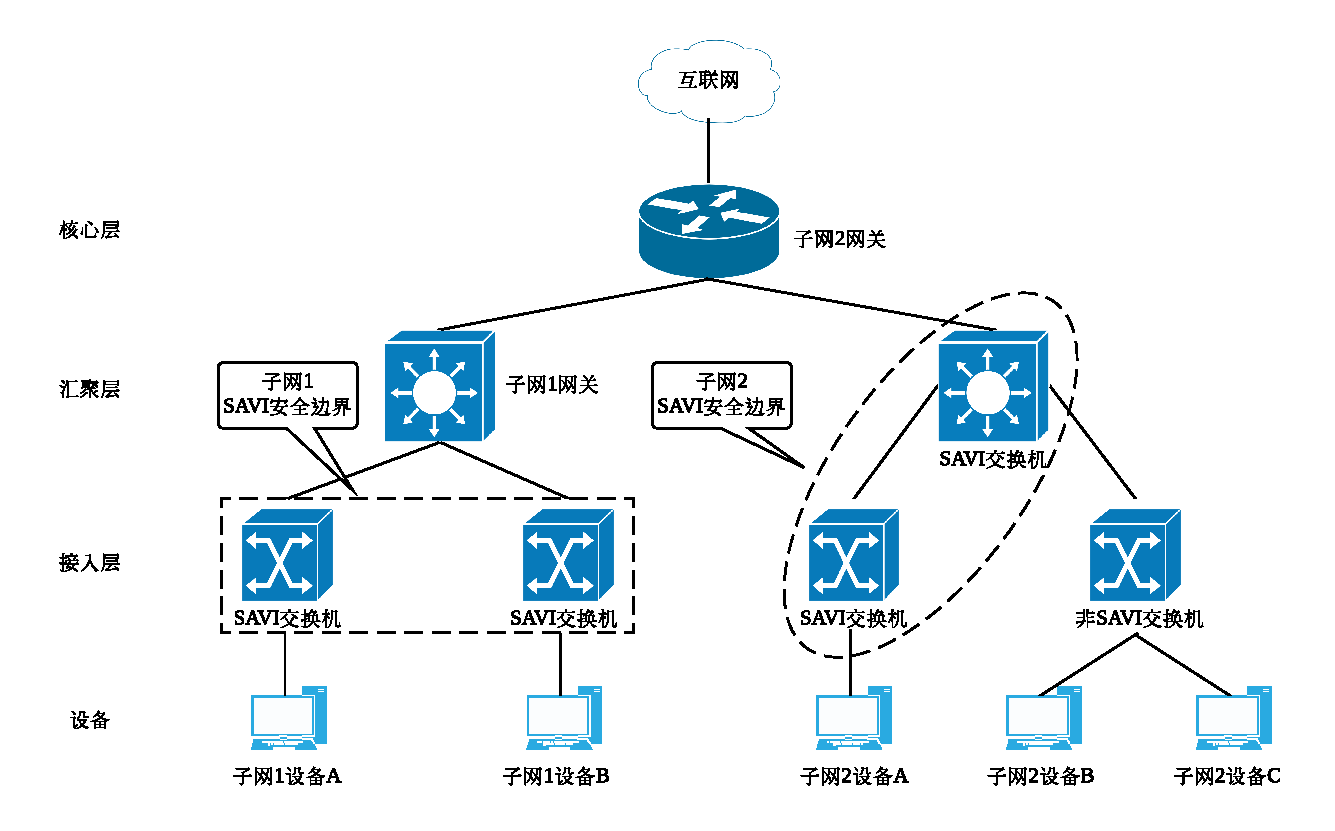
\includegraphics[width=0.9\textwidth]{SAVI_bound.pdf}
        \caption{SAVI安全边界示意}
        \label{fig:SAVI_bound}
      \end{figure}

      此外,在图\ref{fig:SAVI_bound}中,子网2内支持SAVI的接入交换机与汇聚交换机形成了级联的关系,在接入交换机已经对报文进行过滤的情况下,汇聚交换机不必再次进行SAVI绑定表的建立与报文的检查,因此为了在多SAVI交换机级联的场景下避免表项冗余,SAVI技术支持设置SAVI Trust端口,对其下的报文进行信任,不进行控制报文监听和数据报文过滤,从而支持网络的大规模扩展。

    \subsection{自治域内源地址验证}
    \label{survey:sava:intraas}
    自治域内的源地址验证技术需要进行IP地址前缀粒度的伪造报文过滤,避免同一自治域内某一子网的用户使用不属于其所在子网的IP地址向外发送报文的情况发生,其伪造报文过滤粒度在子网级别。目前域内源地址验证技术的研究相对较少,这一方面是由于自治域一般属于同一个管理域,所有接入子网都处于网络管理员的管辖之下,域内源地址伪造的问题不易发生,另一方面也由于可以通过在接入子网网关设备处进行一些简单的配置以进行域内伪造报文的过滤,自治域内源地址验证方案的部署收益不高。

    通过ACL(Access Control List)的手段可在各子网网关处配置对报文源地址进行检查,仅允许使用来自本子网地址作为源IP的报文通过,从而实现不同子网之间的设备不发生源地址伪造。
    uRPF(unicast Reverse Path Forwarding)\cite{uRPF}使用转发表作为过滤表,避免了ACL的手动配置,但其仅适用于对称路由的域内结构,对于需要增强网络可用性而常具有链路备份的组网方式而言容易发生错误丢弃正确报文的假阳性问题。
    SAVO\cite{I-D.tao-savi-savo}基于OSPF协议\cite{RFC2740}学习域内的链路状态并计算合法的报文转发路径,以消除uRPF对对称路由的假设。但自治域内往往不止OSPF一种路由协议,还可能存在手动配置的静态路由,基于OSPF难以获得完整的路由拓扑信息,也可能出现假阳性等问题。
    CPF(Calculated Path Forwarding)\cite{duan2006constructing}通过SNMP\cite{RFC3411,RFC3413}从域内的路由器中收集管理信息数据MIB,从而获取域内的路由信息,并计算域内报文转发的合法路径,生成伪造报文的过滤规则,并通过SSH\cite{RFC4251}配置到各路由器的ACL中,从而减轻手工配置的负担,并消除假阳性等问题。

    \subsection{自治域间源地址验证}
    \label{survey:sava:interas}
    自治域间源地址验证技术是解决跨域源地址伪造问题的验证技术。由于其研究对象涉及多个自治域,自治域间利益难以统一,单一自治域部署源地址验证技术只会增加自治域管理员的运维负担,却没有提供防御来自其他自治域的恶意流量的能力,因而自治域间源地址验证的方案往往缺乏部署激励。根据自治域间源地址验证技术原理的不同,本文将其划分为基于端到端验证思想的方案与基于拓扑验证思想的方案两类。

      \subsubsection{端到端验证类自治域间源地址验证方案}
      \label{survey:sava:interas:tag}
      端到端验证类方案是指基于如下思路的一类技术:通信的自治域双方首先建立相互的信任关系,在发送域间报文前首先在控制平面协商验证域间报文源地址真实性的方法,源自治域的数据平面为出域报文添加根据协商方法生成的保障报文源地址真实性的标签,由目的自治域数据平面根据控制平面传递的信息验证入域报文所携带标签的合法性从而判断源地址的真伪,如图\ref{fig:end_to_end_validation}所示。

      \begin{figure}[ht]
        \centering
        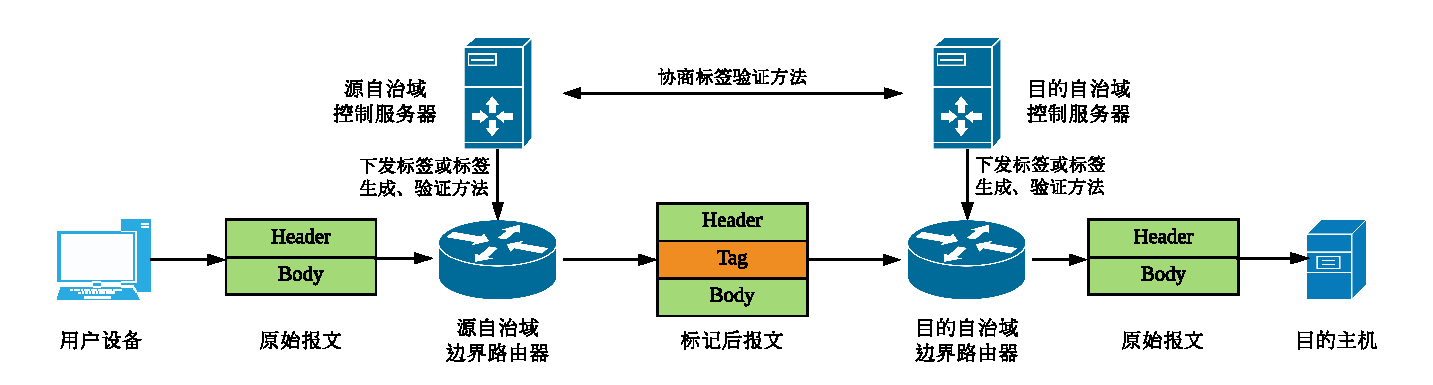
\includegraphics[width=0.9\textwidth]{end_to_end_validation.pdf}
        \caption{端到端验证类自治域间源地址验证方案原理}
        \label{fig:end_to_end_validation}
      \end{figure}

      为实现自治域间端到端的标签验证,自治域的控制平面需要首先建立通信确认对方可信的身份,因而各类方案均不可避免地引入一个安全联盟的概念以确保对方自治域的行为受到一定的约束,同时采用可信的第三方维护自治域控制平面的信息,以使各自治域控制平面之间能够顺利建立通信并确认身份。因此,基于端到端验证思想的自治域间源地址方案拓扑一般如图\ref{fig:end_to_end_validation_topology}所示。可见,维护自治域之间互信关系的可信第三方在端到端验证方案中具有特殊地位,其工作正常与否将直接影响到所有部署了自治域间源地址验证方案的自治域间报文的转发。

      \begin{figure}[ht]
        \centering
        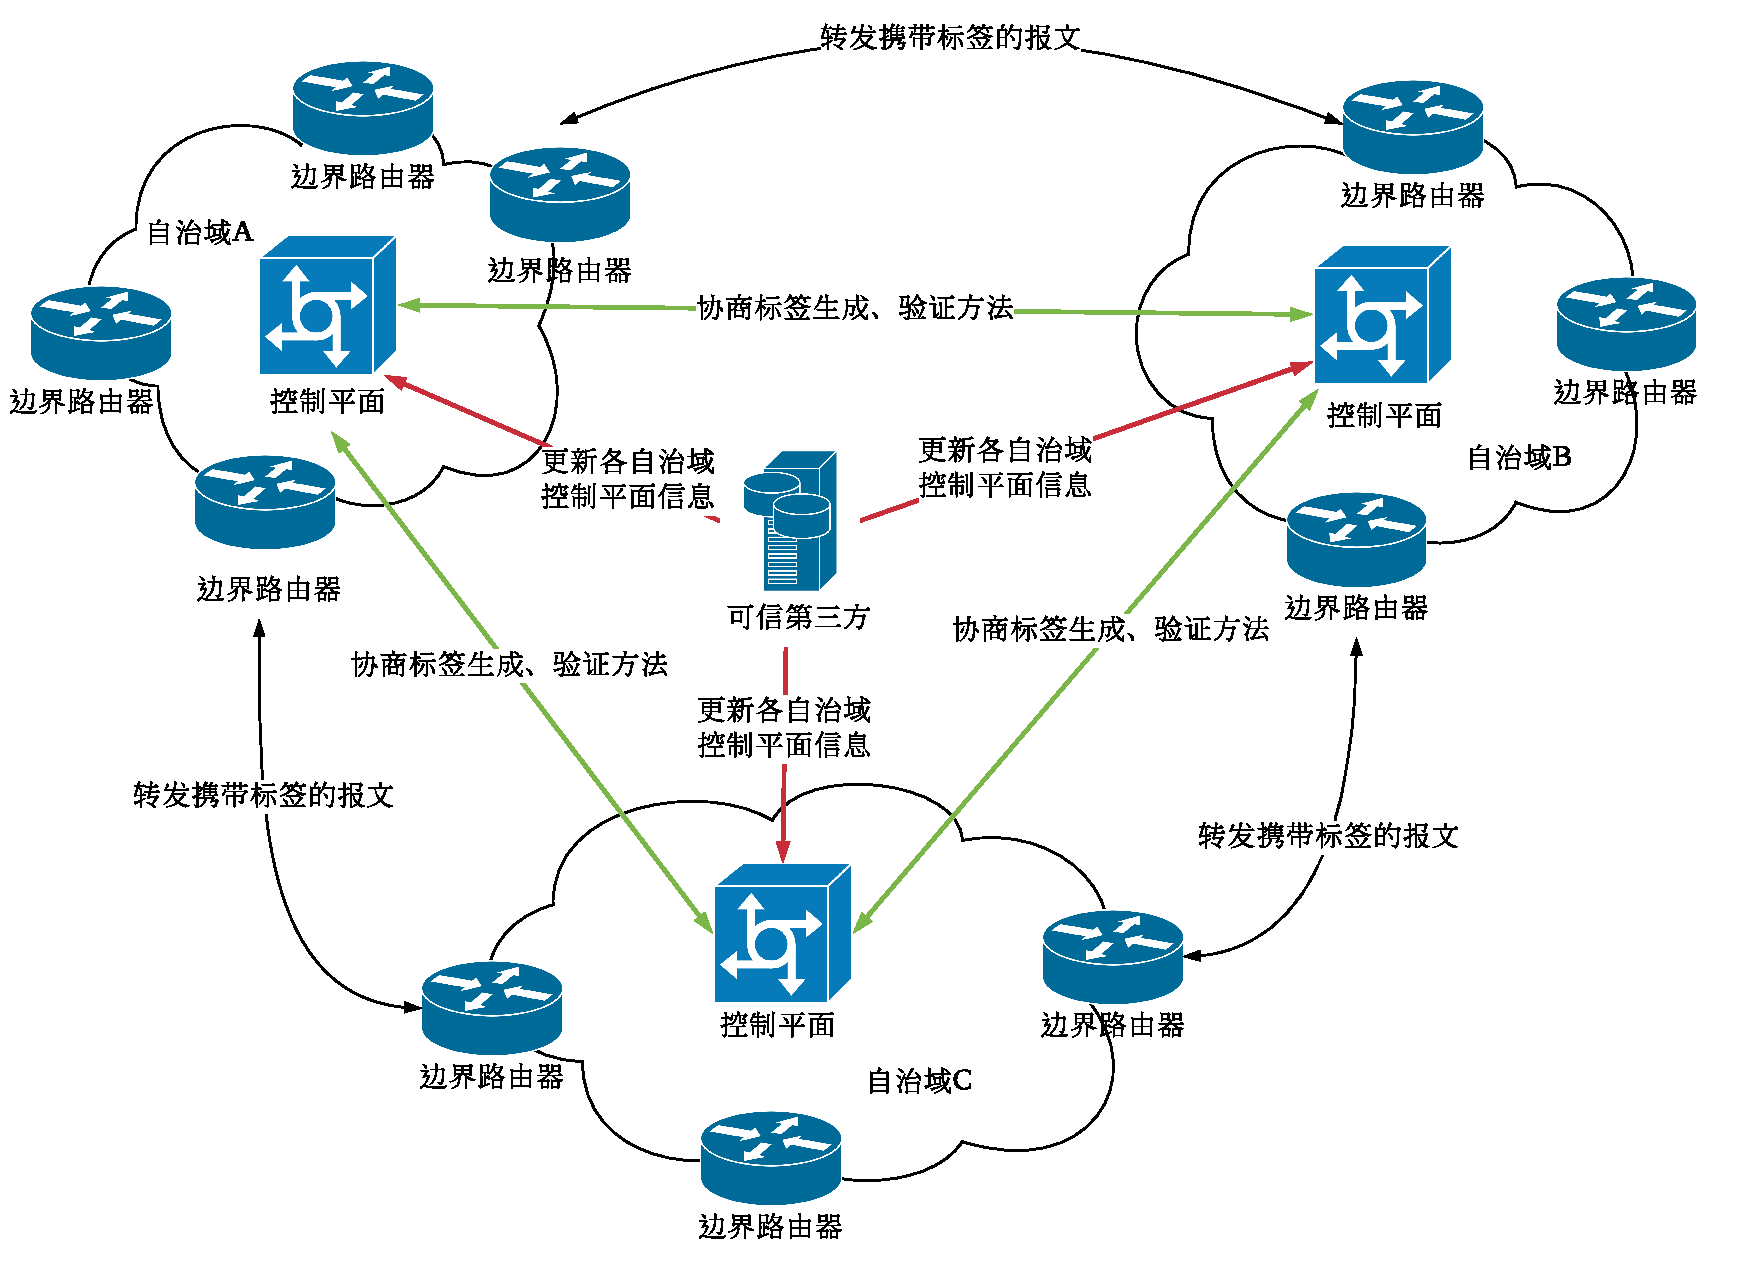
\includegraphics[width=0.7\textwidth]{end_to_end_validation_topology.pdf}
        \caption{端到端验证类自治域间源地址验证方案结构示意}
        \label{fig:end_to_end_validation_topology}
      \end{figure}

      IPSec\cite{RFC2401}中提出的认证头隧道模式在自治域之间建立安全的通信隧道,在完成对端身份校验后,源自治域使用对完整报文进行哈希的方式生成标签并携带在报文中,目的自治域根据协商好的密钥采用同样的哈希算法对报文进行计算并与报文携带的标签进行比较,从而验证完整报文的真实性,其对每个完整报文都进行哈希生成标签的操作,为数据平面带来了较大的性能开销。
      SPM\cite{bremler2005spoofing}采取与IPSec类似的思想生成标签,但其仅对报文的头部进行哈希以降低性能开销,并提出了安全联盟的概念以增强自治域间源地址验证技术的部署激励,即仅有加入安全联盟的自治域才能够享受到自治域间源地址验证技术的安全性保障,从而吸引更多自治域加入安全联盟部署该技术。
      Passport\cite{liu2006efficient}在SPM的基础上,增加了路径检查的功能,要求在报文转发路径上的每个自治域均对报文进行检查,属于一种标签和路径合法性检查并举的方案。这种方式虽然提供了在到达目的自治域前阻断攻击流量的功能,但由于路由动态变化的影响,Passport易导致报文的错误丢弃。
      SMA\cite{shen2008two,bi2009preventing}同样采用基于安全联盟的设计,但使用状态机对数据平面性能做了更进一步的优化,各自治域控制服务器ACS之间定期进行通信协商状态机,而后即采用状态机生成的标签作为报文源IPv6地址真实的背书证据,并通过标签序列的快速变化避免标签被攻击者伪造,避免了数据平面对报文的签名操作。

      总而言之,相较于拓扑验证类自治域间源地址验证方案,端到端类自治域间源地址验证方案的优势主要有:
      \begin{itemize}
        \item 支持增量部署,允许若干自治域先行部署方案并逐步推广。
        \item 安全联盟内自治域间源地址伪造可预防,具备一定部署激励。
        \item 不依赖于网络中运行的其他协议,不受制于依赖协议的安全性。
        \item 不对报文转发拓扑进行假设,不易出现丢弃合法报文的假阳性问题。
      \end{itemize}

      另一方面,端到端验证类源地址验证方案共有的不足之处主要在于:
      \begin{itemize}
        \item 数据平面增加了额外的性能开销。
        \item 控制平面间的协商过程维护较复杂,易发生错误或遭受攻击。
        \item 需引入额外的信任基础维护自治域间通信所需信息,且其功能直接影响到所有跨域报文的转发。
        \item 对于伪造源地址的恶意流量仅能在目的自治域进行阻断,无法消除转发路径上网络资源的损耗。
      \end{itemize}

      \subsubsection{拓扑验证类自治域间源地址验证方案}
      \label{survey:sava:interas:path}
      拓扑验证类的自治域间源地址验证方案是指这样一类技术:网络中各自治域通过一定手段学习跨域报文的合法转发路径,在报文由源自治域路由至目的自治域的过程中,由所经过的各自治域节点对报文转发路径的合法性进行检查,提前过滤源地址与合法转发路径不匹配的报文,如图\ref{fig:topology_validation}所示。

      \begin{figure}[ht]
        \centering
        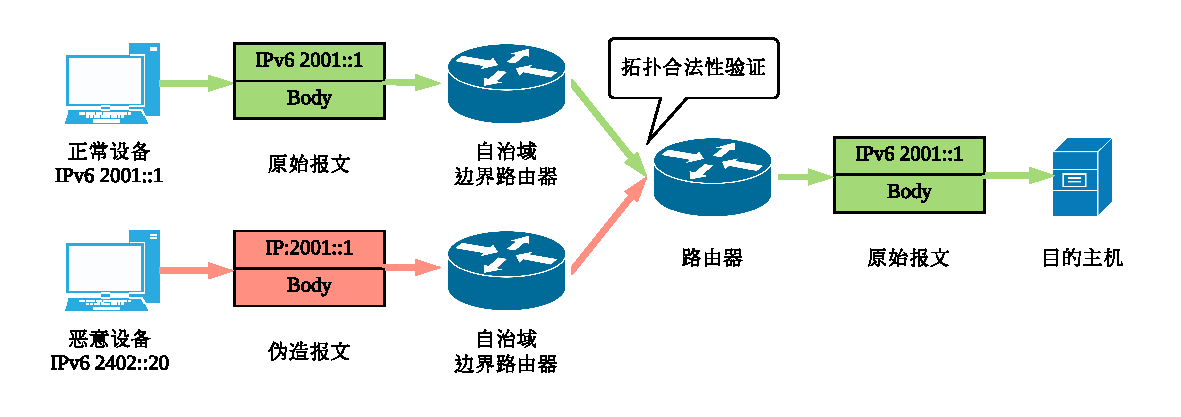
\includegraphics[width=0.9\textwidth]{topology_validation.pdf}
        \caption{拓扑验证类自治域间源地址验证方案原理}
        \label{fig:topology_validation}
      \end{figure}

      IEF(Ingress/Egress Filtering)\cite{RFC2827}通过在各自治域的边界进行出口检查,过滤伪造源IP地址的报文,仅允许本自治域的源IP地址报文转发,在转发路径的起始点进行恶意流量的拦截。但IEF仅能规范自治域自身的行为,而难以预防来自其他自治域的攻击,且需要进行手动配置、增加运维难度,因而难以带来部署激励。
      uRPF\cite{uRPF}针对IEF运维困难的问题,以残桩自治域的拓扑结构作为假设前提,将IEF中过滤伪造报文的关口上移至残桩自治域所上连的自治域,利用BGP协议提供的拓扑信息,自动配置来自残桩自治域的报文的过滤规则,减轻了手工配置的难度与易出错性,但由于互联网环境的复杂与各自治域对可用性的考虑,其残桩自治域的假设不具备普适性。
      IDPF(Inter-Domain Packet Filters)\cite{duan2006constructing}通过假设报文转发路径与BGP Update宣告的路径一致,根据IP前缀路由对报文的不合法转发路径进行过滤。IDPF拓展了方案的使用范围,但其假设过于理想,而网络中存在大量非对称路由,且报文的转发路径很可能随着网络环境的改变而发生实时变化,因此容易造成合法报文的错误过滤。
      SN(Selection Notice)\cite{lijun2006bgp}通过拓展BGP协议,为其新增路由选择公告的报文以在自治域路由规则更新时将其告知对端自治域,路径上的各自治域也通过学习路由选择公告报文来学习新的路径过滤规则。这种方式使报文转发路径中的任一自治域均有对报文进行验证的能力,但其受制于BGP自身的安全,同时其功能的正确运作要求该技术的全局部署,无法支持增量部署的方式。
      SAVE(Source Address Validation Enforcement)\cite{li2002save}设计了一种独立于路由协议的SAVE协议来实现路由路径探测的功能,其通过周期性发送SAVE Update报文建立自治域的入向树,自治域边界路由器则根据入向树的结构生成用于源地址验证的入向表,这种方式解耦了与路由协议的绑定,消除了其他协议带来的依赖安全性,但其正常运作同样依赖于全局部署,并且实现方式过于复杂,难以进行实际的部署。

      总而言之,基于拓扑合法性检查的源地址验证方案虽可以提前过滤伪造源地址的流量,尽可能地增大部署方案所带来的经济收益,但也存在共有的不足之处:
      \begin{itemize}
        \item 拓扑验证规则难以建立;
        \item 许多方案与BGP协议存在耦合,受制于BGP安全性;
        \item 验证规则易受路由动态性的影响,造成报文的错误过滤;
        \item 难以过滤符合拓扑验证规则的源地址伪造报文;
        \item 难以支持增量部署,缺乏推广的可行性。
      \end{itemize}

  \section{IPv6地址生成方案的研究}
  \label{survey:generation}
  由于IPv6允许采取SLAAC方式配置地址,因此网络设备需要能够高效地生成IPv6地址的方案,而IPv6巨大的地址空间,一方面为IPv6地址资源的管理和监测带来了挑战,另一方面也为IPv6地址携带除寻址作用外更丰富的信息带来了可能。IPv6单播地址可分为IPv6子网前缀与接口标识两个组成部分\cite{RFC4291},本节主要综述研究如何生成接口标识的相关方案,其他的地址生成方案例如SIIT\cite{RFC2765}、IVI\cite{RFC6219}等主要研究从IPv4到IPv6地址的翻译过渡技术,而非用户接入IPv6网络时的地址生成方案,因此不在本文的讨论范畴以内。目前已有多种IPv6地址的生成方案被提出,各类方案往往都利用设备或用户身份等信息生成不易冲突的接口标识,但在隐私保护、网络管理、用户审计、路由聚合等方面做了不同的取舍。

  RFC 2464\cite{RFC2464}中提出采用根据IEEE 802定义的48位MAC地址生成EUI-64标识符作为IPv6地址的接口标识。这种生成方式较为简单,但其生成的IPv6地址不发生变化,与用户接口的二层地址相绑定,易造成隐私泄露的问题。
  RFC 4941\cite{RFC4941}针对这一问题提出了临时地址方案,使用加密算法对EUI-64标识符进行哈希后生成接口标识,同时定期更换所生成的IPv6地址。这种方式在一定程度上保护了用户设备的隐私,但增加了网络管理的复杂性。
  RFC 7217\cite{RFC7217}为减轻临时地址方案所带来的网络管理复杂性,提出了一种语义不透明的接口标识生成方法,能够保护用户隐私并提供较为稳定的IPv6地址。
  上述方案均未充分利用IPv6地址空间巨大的优势,使IPv6地址携带更多的语义信息。
  GIRO\cite{oliveira2007geographically}关注IPv6地址的路由聚合问题,提出一种根据地理位置和网络服务提供商对IPv6地址进行生成的方案,以实现相同地理位置、同一运营商内部能够进行较好的路由聚合。
  NIDTGA地址生成方案\cite{liu2015building}针对用户溯源功能进行研究,充分利用IPv6地址空间广阔的优势在接口标识中嵌入对称加密后的用户网络身份标识与时间信息,可在保护用户隐私的同时实现根据IPv6地址追溯用户身份的功能,为建设对恶意攻击者的威慑手段提供了有力支持。

  \section{用户身份认证与溯源技术}
  \label{survey:identity}
  
      \subsection{用户身份认证技术}
      \label{survey:identity:authenticate}
      对用户在接入时进行身份认证的技术一般可分为三类:二层准入认证技术、三层准入认证技术以及客户端技术。
      
      二层准入认证技术的特点是用户设备与认证控制设备之间通过二层的数据帧进行认证信息的传递,用户设备配置IP地址必须发生在用户完成认证之后,在没有完成身份认证前,网络层及以上的报文是无法通过认证控制设备的。PPPoE认证\cite{RFC2516}采用PPP协议通过以太网实施用户接入,为以太网帧提供身份验证的功能,用户设备通过点对点协议与认证控制设备进行链路协商、用户认证信息的提交,由认证控制设备本地认证或通过RADIUS协议去AAA服务器处完成认证。PPPoE认证方式的缺点是需要安装特定的客户端软件,并且其封装代价高,用户认证效率较低。802.1X\cite{ieee802ieee}是更为广泛使用的二层准入认证方式,与PPPoE类似,用户设备通过链路层数据帧与认证控制设备进行通信,但其不需要进行基于以太帧的封装,因此认证的开销较小。本文后续将重点研究基于802.1X作为二层准入认证手段的用户身份识别与溯源系统设计,在此对802.1X的工作原理进行详细介绍。
      
      802.1X认证过程一般涉及用户设备、认证控制设备、AAA服务器三个角色,其中用户设备与认证控制设备之间使用EAP协议帧进行通信,认证控制设备一般将用户的EAP帧封装为RADIUS报文,发送至AAA服务器进行认证。配置了802.1X认证的接入设备,如接入交换机或无线AP等,对于每台用户设备的MAC地址,将虚拟出两个虚拟端口,其中一个被称为非受控端口,仅允许802.1X认证的EAP帧通过,另一个则称为受控端口,用于控制用户其他报文的转发。在设备认证通过前,其仅能通过非受控端口发送EAP协议帧进行用户身份认证。一个典型的认证过程如图\ref{fig:802.1X_authentication}所示:
        \begin{enumerate}[1{)}]
          \item 用户设备连接认证控制设备,建立新的连接,用户设备的802.1X客户端发送EAPOL Start帧,发起802.1X认证的流程。
          \item 认证控制设备处根据用户设备MAC地址对其进行标识,向其回复EAP Request Identity帧,请求使用该设备的用户身份。
          \item 用户在操作系统自带的802.1X客户端上填写用户名与密码,将用户名携带在EAP Response Identity帧中回复认证控制设备;认证控制设备提取EAP Response Identity中的用户名,将其与原EAP帧均封装为RADIUS Access Request报文中的属性后,采用RADIUS协议将认证报文发送给AAA服务器请求认证。
          \item AAA服务器将根据RADIUS报文中携带的用户名属性,提取用户名查询用户数据库,确认存在后向认证控制设备回复RADIUS Access Challenge报文,其中包含回复用户设备的EAP Request帧,用于说明希望用户设备加密用户密码等信息的EAP方法;认证控制设备解封装RADIUS Access Challenge报文,将EAP Request帧转发给用户设备。
          \item 用户设备若同意AAA服务器与之协商的EAP方法,则根据该方式加密用户密码,将密文携带在EAP Response帧中发送给认证控制设备;认证控制设备将其封装在RADIUS Access Request报文中发送至AAA服务器。
          \item AAA服务器收到RADIUS报文后,检查其中携带的EAP Response帧中的密文,与用户数据库中用户密码根据相同加密方式生成的密文相比较,若相同,则回复RADIUS Access Success报文;认证控制设备将提取RADIUS Access Success报文中的EAP Success帧,将其转发给用户设备,并打开用户设备MAC地址对应的受控端口,允许除EAP帧以外的其他类型流量通过。
        \end{enumerate}
    
        \begin{figure}[ht]
          \centering
          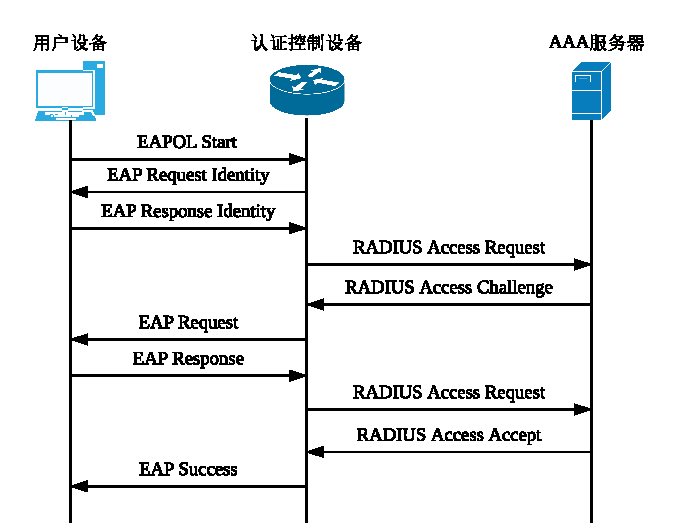
\includegraphics[width=0.8\textwidth]{8021X_authentication.pdf}
          \caption{802.1X认证时序}
          \label{fig:802.1X_authentication}
        \end{figure}
        
      802.1X认证手段的优势在于认证过程安全、认证效率高、设备广泛支持、建网成本低、对无线终端漫游支持较好,但由于其二层认证的特性,仅能支持针对在线时长的计费,难以支持对用户流量的计费。
      
      三层准入认证手段一般通过Web Portal提交用户认证信息。用户首先完成IP地址配置,然后在发送ARP、ND请求过程或通过浏览器访问网络时,触发认证控制设备的认证流程。认证控制设备将用户流量重定向至Web Portal的认证页面,在用户提交用户名、密码等信息完成认证后,Web Portal认证系统向认证控制设备下发用户对应的流量规则,允许用户设备对应的IP地址流量访问外部网络,其一般流程如图\ref{fig:web_portal_procedure}所示。目前Web Portal认证虽然在实际网络中广泛使用,但均为厂商内部实现,并未形成统一的国际标准。
      
      \begin{figure}[ht]
        \centering
        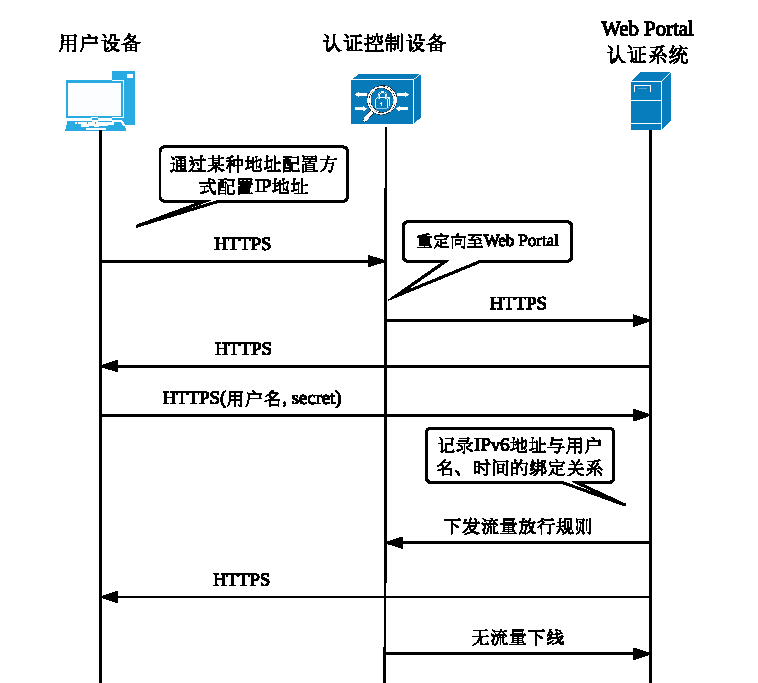
\includegraphics[width=0.8\textwidth]{web_portal_procedure.pdf}
        \caption{Web Portal认证时序}
        \label{fig:web_portal_procedure}
      \end{figure}
      
      Web Portal认证手段的优势在于不依赖于客户端、便于用户身份与IP地址的绑定、能够支持流量计费,但其安全性较弱,与用户的连接性差,不能很好地支持用户漫游的场景,组网的成本高,并且认证流程与交互信息没有规范化,未形成国际标准。
      
      客户端认证手段则是指一类在用户设备上安装特定软件以实施用户接入功能的身份认证方式。一般而言,客户端认证均是利用定制客户端替代操作系统内核某一模块功能,在其原生模块功能之上增加一定的功能扩展,如用户身份认证、设备安全性检查等,以实现个性化定制认证流程的功能。这种方式灵活性较强,可能可以提供更强的安全性,但其开发工作量大,推广部署困难,并且其私有化程度高,引入新的安全问题的风险更大。
  
      \subsection{用户身份溯源技术}
      \label{survey:identity:trace}
      目前根据IP地址对用户身份进行追溯的方法主要有两种。一种是在利用Web Portal进行用户身份认证的网络中常见的IP地址与用户身份绑定方案,另一种则是NIDTGA地址生成方案提出的用户身份溯源方法。
    
      Web Portal进行用户身份与IP地址绑定的溯源方案原理比较简单,由于用户认证时需要使用IP地址访问Web Portal网站,因此可以轻易地将用户IP地址与用户认证的身份关联并存储以支持后续的溯源。其能够支持各种IP地址配置方式,但为实现溯源功能必须存储所有历史绑定记录,存储开销较大,并且在IP地址资源进行时分复用的情况下,仅凭IP地址难以确定实际的用户身份,必须配合IP分组的时间信息,为用户身份的溯源带来困难。此外,其方案限定了Web Portal认证的方式,在无线网络发展繁荣的今天难以良好地支持无线终端的移动性要求,而在采用二层准入认证的网络中又难以实现IP地址与用户身份的绑定,不具备较好的推广能力。
    
      NIDTGA地址生成方案\cite{liu2015building}在用户认证时通过IDEA对称加密的方式为其生成嵌入了用户身份与认证时间的IPv6地址,在用户请求配置地址时将其配置给用户设备。在有用户身份溯源需求时,使用密钥更新历史对待追溯的IPv6地址进行解密,以获得用户身份信息,其具体原理如图\ref{fig:NIDTGA_procedure}所示:
      \begin{enumerate}[1{)}]
        \item 组织管理员根据用户在现实生活中的身份标识(如身份证号、学号等)为用户生成一个长度为40位二进制的用户网络身份标识NID。
        \item 用户所在组织的管理域为用户生成IPv6地址时,将NID与当前的时间信息拼接成一个长度为64位二进制数的原文,采用IDEA加密方法根据某一个组织管理员设定的密钥加密获得一个长度为64位二进制数的密文。
        \item 将密文作为接口标识,与用户设备所在子网的IPv6子网前缀拼接,形成用户设备的IPv6地址。
        \item 追溯时,审计方首先根据IPv6地址前缀确定用户所在的组织,获取该组织使用过的IDEA密钥历史。
        \item 根据组织IDEA密钥历史,从最新的密钥开始,按照历史记录往前逐一使用当前密钥对用户IPv6地址的接口标识进行解密,从解密获得的64位原文中提取时间信息。
        \item 比较提取的时间信息与当前解密用密钥的有效时间,若时间信息位于密钥的有效时间内,则说明该IPv6地址接口标识确实由该密钥加密生成,提取接口标识原文中的NID段获得用户身份标识NID。
      \end{enumerate}
    
      \begin{figure}[ht]
        \centering
        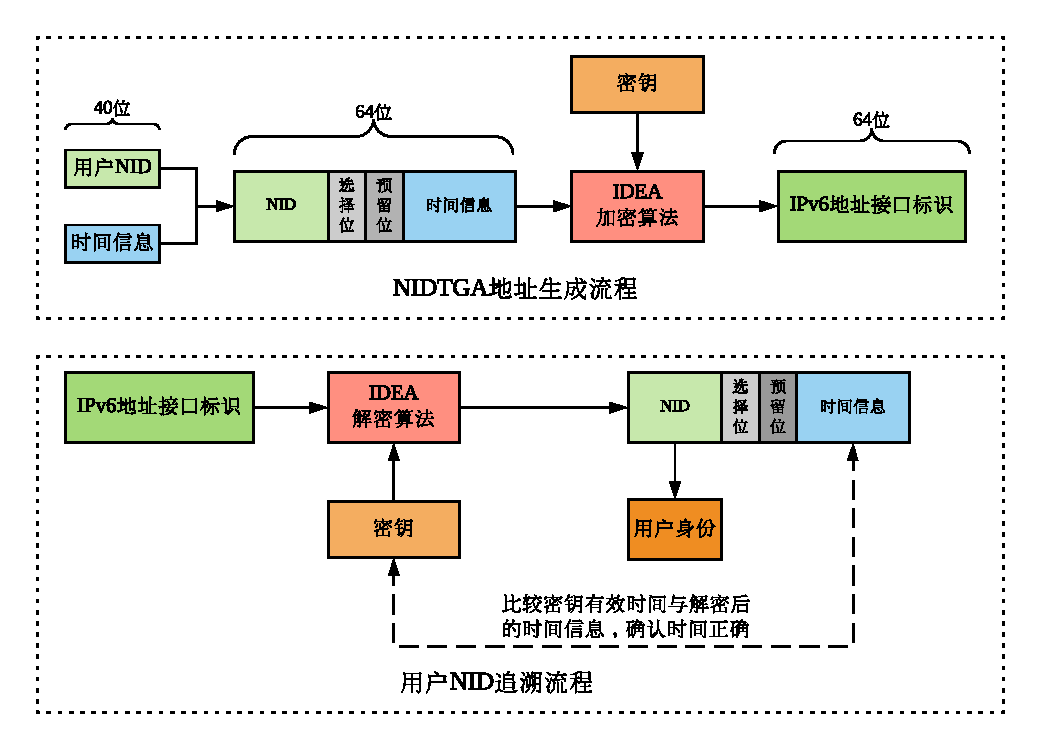
\includegraphics[width=0.9\textwidth]{NIDTGA_procedure.pdf}
        \caption{NIDTGA地址生成与追溯过程}
        \label{fig:NIDTGA_procedure}
      \end{figure}
    
      NIDTGA地址生成方案将用户身份与时间信息均携带在IPv6地址内部,无需进行IPv6地址与用户身份绑定关系的存储,节省了存储开销,在溯源时无需确定恶意分组的时间信息,避免了身份溯源的错误,增添了溯源能力的便利。其统一的用户身份标识NID设计,也为跨管理域的用户身份统一溯源奠定了基础,有利于该技术的推广。但是,其未对接入网络中复杂的用户认证与地址配置的结合方式加以详细的考虑,因此采用NIDTGA地址生成方案的用户身份识别与溯源系统在实际网络环境中的设计与实现仍亟待研究。

  \section{区块链的相关研究}
  \label{survey:blockchain}

    \subsection{区块链原理}
    \label{survey:blockchain:theory}
    区块链的本质为一个分布式数据库,其记录的数据内容被分散地备份在区块链网络中每一个完整的区块链节点上,所有节点之间通过共识算法达成对数据库中数据的共识。其记录数据的方式不同于传统的关系型数据库支持数据的本地修改,而是更接近追加型的NoSQL,仅能向其中写入新的数据而无法对已写入区块链的数据进行更改。与普通的追加型NoSQL数据库有别的是,区块链将数据进行分块,存储为首尾相连的链表格式,并使用密码学技术确保攻击者难以承受篡改数据的代价以规避数据被篡改的可能。向区块链中写入新数据的过程并非分布式系统中常用的主从复制模式,而是往往通过一些资源拥有证明的方法来处理数据写入的权力分配,当攻击者无法占有区块链网络中大部分的资源时,它就无法垄断区块链中数据写入的权力,因此可以被应用于拜占庭情况下的网络环境中。由于区块链最初诞生于加密货币领域,被用于交易的记账,因此人们更多地称其为分布式账本。

    一个典型的区块链结构如图\ref{fig:blockchain_structure}所示。整个区块链呈一个链表状的结构,链表中每个节点都是一个区块(Block),区块之间依次相连,新的数据将组成一个新的区块添加到链表的末尾,指向先前的区块。以比特币的区块链为例,其每一个区块分为区块头(Block Header)与区块体(Block Body)两部分。区块头中记录了区块版本、前一区块的哈希值、Merkle树\cite{merkle1987digital}根节点、时间戳以及随机数答案等,区块体中记录了这一区块出块过程中发生的交易(Transaction)数量和每笔交易的信息。

    \begin{figure}[ht]
      \centering
      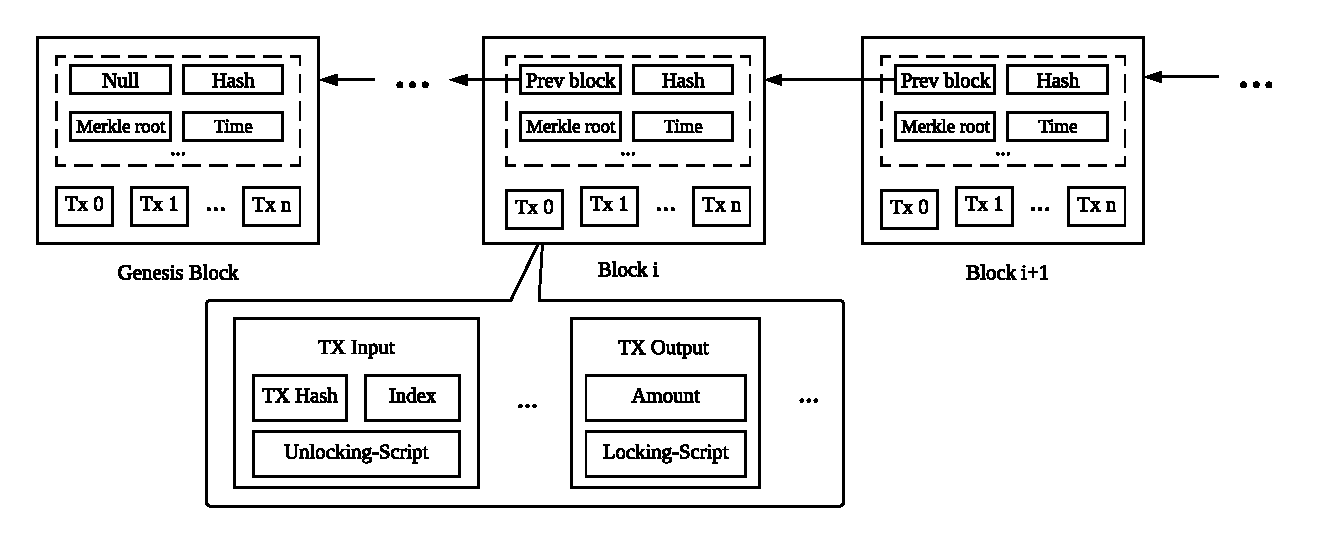
\includegraphics[width=0.9\textwidth]{blockchain_structure.pdf}
      \caption{区块链结构示意}
      \label{fig:blockchain_structure}
    \end{figure}

    用户要与区块链进行交互,首先需要创建其钱包。所谓钱包,其实就是一个公私钥对,钱包的地址由公钥经过一系列数字签名运算后得到。区块链使用公私钥对来确保交易的合法性。当用户有新的数据想要写入区块链时,其首先使用私钥对包含了数据的交易进行签名,然后通过区块链节点广播到整个区块链网络中。网络中的其他节点将使用交易发起者的公钥对交易签名进行验证,从而保证交易在传播途中没有遭到篡改。

    当有新的数据需要写入区块链中时,区块链网络中的各个节点会通过一种名为挖矿(Mining)的方式对新区块中的内容达成共识,参与挖矿的节点被称为矿工(Miner)。挖矿过程中采用的共识算法有非常多种,但最广为人知且得到良好实践的一种即为比特币所采用的工作量证明(Proof of Work,PoW)方法。以比特币为例,其工作原理如下:
    \begin{enumerate}[1{)}]
      \item 矿工节点收集到足够多的合法交易后,其将这些交易打包为一个区块,并生成包含前一区块哈希值、本区块所包含交易的Merkle树根、时间戳等信息的区块头,并开始计算如下的工作量证明难题:寻找区块头中的随机数答案nonce值,使得将80个字节的区块头作为输入送给SHA256\cite{burrows1995secure}算法进行哈希后,所得到的答案小于区块链网络当前的目标值。当前目标值由式\eqref{eq:blockchain_pow_adjustment}进行调整。设区块链网络设定的最大目标值为$M$,当前难度值为$d$,则目标值$o$由式\eqref{eq:blockchain_target}确定。比特币网络每产生2016个区块即会根据其运行状态调整难度值$d$,设原本的难度值为$d'$,过去生成2016个区块的总时间为$t$,则新的难度值$d$由
      式\eqref{eq:blockchain_difficulty}确定,以保证整个比特币网络始终以约每十分钟一个区块的速度产生区块。
      \begin{subequations}
        \label{eq:blockchain_pow_adjustment}
        \begin{align}
          o &= \frac{M}{d} \label{eq:blockchain_target}  \\
          d &= d' * \frac{t}{2016*10} \label{eq:blockchain_difficulty}    
        \end{align}
      \end{subequations}
      \item 矿工将持续不断地尝试改变nonce值并进行SHA256计算,直至寻找到一个满足SHA256$(block\_header) <= o$的nonce值。一旦找到,矿工立即将其填入区块头中的对应字段,向比特币网络广播新区块。
      \item 网络中其他节点收到广播的新区块时,将对其区块头进行校验,检查内容包括该区块头所包含的哈希值是否与其高度的前一个区块一致、宣告的答案是否满足当前网络的工作量证明约束等,然后验证新区块中每一笔交易的合法性,若全部校验通过,则节点将该新区块加入到自身维护的区块链中。
    \end{enumerate}

    由于区块链中采用链表的形式对数据进行组织,每一个区块中都包含有前一区块数据的哈希值,因此如果攻击者想要欺骗整个区块链网络,使其他诚实的区块链节点对某一区块中的伪造数据达成共识,其需要对自该区块开始往后的全部区块重新进行工作量证明的计算,而工作量证明难题确保了挖矿能力与节点的算力成正比,因此没有掌握全网一半以上算力的攻击者无法对已经形成共识的区块链数据进行篡改,从而保障了区块链中数据不受篡改的特性。

    同时,由于区块链中数据的全量副本均分布在每一个区块链节点上,其天然拥有容灾备份的优势,可以极大提高数据的可靠性。

    \subsection{区块链技术的发展}
    \label{survey:blockchain:development}
    在比特币网络中,区块链仅仅作为一个分布式账本对比特币转账交易进行记录,尽管其能够执行一些脚本命令,但所支持的功能是十分受限的,因而难以在其上构建除加密货币外的其他应用。

    针对这一问题,以太坊\cite{wood2014ethereum}提出了以太坊虚拟机(Ethereum Virtual Machine,EVM)与图灵完备的Solidity语言。使用Solidity语言编写的智能合约能够实现用户自定义的应用逻辑,并被部署到以太坊网络在EVM内部执行。由于这种应用分散于整个以太坊网络的各个节点,因而常被称为分布式应用(Distributed App,DApp)。当用户发起交易时,交易可以定义创建合约、调用合约、向合约转账等功能的各种逻辑。由于合约的执行需要消耗节点的资源,因此为了使自己的交易能够被矿工节点打包入区块中,用户需要向矿工节点支付一种名为Gas的费用,以用户愿意支付的以太币(Ethereum,ETH)价格为单位进行衡量。在EVM内部,每一条指令的执行都有其对应消耗的Gas数量,矿工节点将根据用户交易中提供的价格来计算将交易打包进区块所要收取的Gas总价。每一个以太坊节点中的区块链都会记录智能合约的代码与状态,当节点需要验证新的区块时,对于区块中有合约交互的交易,以太坊将根据交易顺序在EVM中依次执行交易中调用的合约逻辑,若出现代码执行错误或消耗的Gas总量超出用户交易规定的上限时,新区块的验证失败,EVM将终止智能合约的执行,并将区块链回滚到未验证新区块之前的状态。以太坊的诞生,使区块链的跨领域应用成为可能,引发了世界范围内开发者在其上构建DApp的热潮,形成了繁荣的以太坊生态。但是,以太坊仍存在以下缺陷:
    \begin{itemize}
      \item 目前的以太坊网络仍采用PoW共识方法,尽管可以根据难度值的调整缩短达成共识的时间,但其上智能合约的调用仍是异步的过程,难以媲美传统应用同步调用的性能;
      \item 在以太坊上构建DApp必须使用Solidity这一领域限定语言,而不支持类似于Java、Go等非领域限定的高级语言,对DApp的开发造成了一定的壁垒。
    \end{itemize}

    与比特币、以太坊不同,超级账本技术\cite{dhillon2017hyperledger}致力于采用区块链技术解决非公开网络中的数据安全问题,其应用场景并非完全不可信的参与方,而是互相之间具有信任基础的联盟体。因此其在区块链的性能与数据安全性之间做了一定取舍,并采用容器技术支持了通用高级语言的执行。Fabric\cite{androulaki2018hyperledger}采用Kafka\cite{thein2014apache}或Raft\cite{ongaro2014search}共识算法替代了PoW,优化了共识算法的性能,但舍弃了对恶意节点接入的防御能力。其提出了账本节点、排序节点等多种节点角色,支持节点之间创建Channel,在同一个Fabric网络中构建多个分布式账本,以更好地满足联盟链场景下的需求。Fabric对高级语言的支持更为充分,支持开发者使用Java、Go与Node.js开发分布式应用并在容器Docker中运行,降低了区块链开发的门槛。Besu\cite{Besu}在以太坊的基础上引入了IBFT、Clique等权威证明的共识机制,并为联盟链和私有链场景设计了更为友好的以太坊客户端以适应企业的需求。Indy\cite{Indy}为区块链上的数字身份互操作场景提供了可重用组件的解决方案。Sawtooth\cite{Sawtooth}设计了一种灵活的模块化区块链体系结构,支持用户应用在无感知的情况下可自由地替换底层区块链组件,支持实用拜占庭算法(Practical Byzantine Fault Tolerance, PBFT)\cite{castro1999practical}与经过时间证明算法(Proof of Elapsed Time,PoET)\cite{rilee2018understanding}。超级账本技术对于企业联盟或私有场景提供了比以太坊更为丰富的工具与功能支持,并且往往都支持非领域限定的高级语言进行开发,但其一般采用非PoW的共识算法,虽提升了共识效率,但存在一定程度的中心化特点,削弱了对数据真实性的保护。

  \section{本章小结}
  \label{survey:summary}
  本章从IPv6地址配置方式开始,对实现和部署用户身份识别与溯源系统所需要支持的地址配置场景进行了全面的介绍。同时,对作为用户身份识别与溯源系统依赖基础的源地址验证技术相关研究进行了讨论,指出了接入子网SAVI技术与自治域间端到端类验证方案存在的一些问题。然后分析了各种IPv6地址生成方案的侧重点,介绍了目前唯一一种以用户身份溯源为目的设计的NIDTGA地址生成方案。接着介绍了目前网络中常见的用户身份认证手段与身份溯源方案,讨论了传统的IPv6地址与用户身份绑定方式的问题,说明了采用NIDTGA方案实现用户身份识别与溯源系统的必要性。最后介绍了区块链技术的原理和发展,启发了本文使用区块链提升域间源地址验证技术与用户身份识别与溯源系统跨组织部署时的安全性,并为开发实现时的区块链平台选择提供了参考。



